\documentclass[11pt]{beamer}

\usetheme{metropolis}

\usepackage{graphicx}
\usepackage{physics}
\usepackage{adjustbox}
\usepackage{caption}
\usepackage{chemformula}
\usepackage{quoting}
\usepackage[style=chem-angew,backend=bibtex]{biblatex}
\bibliography{references}
%
% Choose how your presentation looks.
%
% For more themes, color themes and font themes, see:
% http://deic.uab.es/~iblanes/beamer_gallery/index_by_theme.html
%
\mode<presentation>
{
  \usetheme{default}      % or try Darmstadt, Madrid, Warsaw, ...
  \usecolortheme{default} % or try albatross, beaver, crane, ...
  \usefonttheme{default}  % or try serif, structurebold, ...
  \setbeamertemplate{navigation symbols}{}
  \setbeamertemplate{caption}[numbered]
  \setbeamerfont{footnote}{size=\tiny}
} 

\usepackage[english]{babel}
\usepackage[utf8]{inputenc}
\graphicspath{{image/}}

\AtBeginSection[]{
\begin{frame}{Outline}
  \tableofcontents[currentsection]
\end{frame}
}

\title{Chapter 8: Chemical Bonding}
\institute{Chemistry Department, Cypress College}
\date{Nov 14, 2022}

\begin{document}

\begin{frame}
  \titlepage
\end{frame}

\begin{frame}{Class Announcements}
  \textbf{Lab}
  \begin{itemize}
  \item Experiment 18 Boyle's Law
  \item Reminder - Need $70\%$ of laborator points to pass
    the course
  \end{itemize}

  \textbf{Lecture}
  \begin{itemize}
  \item Finish up Ch 8 and begin Ch 9
  \item Go over homework 10 (EC for students who present)
  \item Quiz and Homework assignment released Fri, Nov 18th at 3pm
  \end{itemize}
\end{frame}

\section{Review: Chemical Bonds}

\begin{frame}{What are Chemical Bonds?}
  \begin{center}
    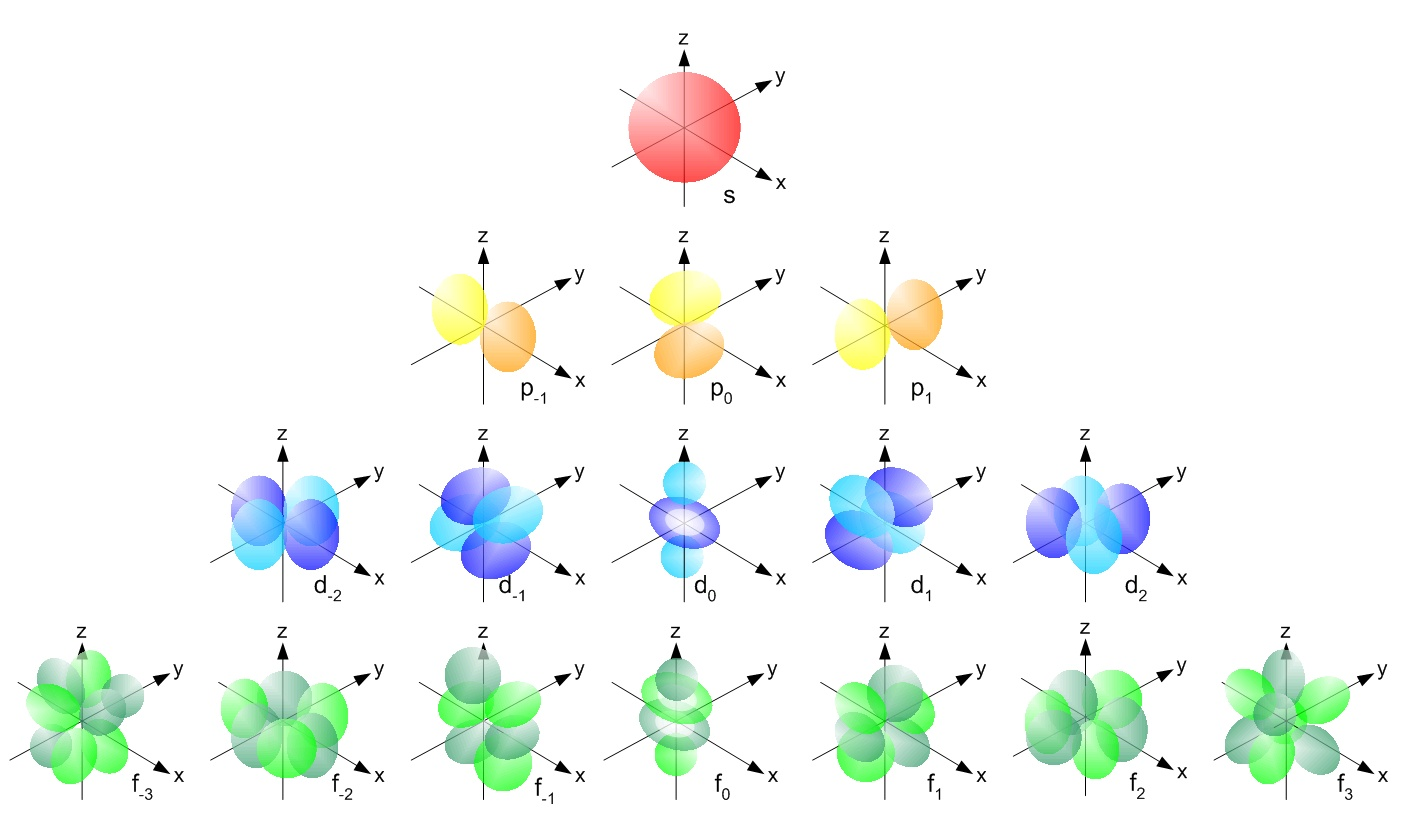
\includegraphics[width=0.8\linewidth]{single_elect_orb}
  \end{center}
  \textbf{Bonds are made up of atomic orbitals}
  \begin{itemize}
  \item Overlap of atomic orbitals lead to the formation of molecular
    orbitals (same energy and specific orientation)
  \end{itemize}
\end{frame}

\begin{frame}{Example with p-orbitals}
  \centering
  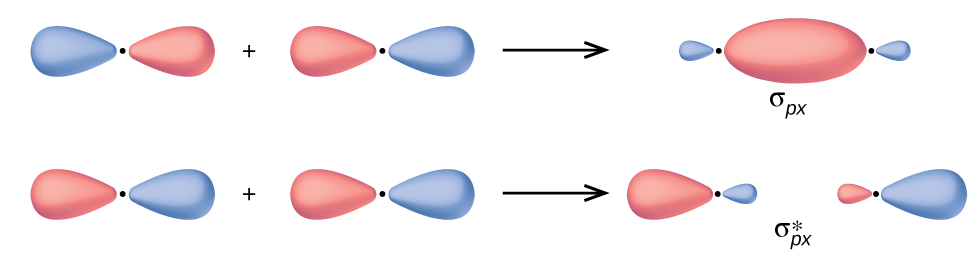
\includegraphics[width=\linewidth]{p_sigma}
  \begin{itemize}
  \item Depending on the orientation, p-orbitals
    will form a bond
  \end{itemize}
\end{frame}

\begin{frame}{Electronegativity: Tug-of-War}
  \centering
  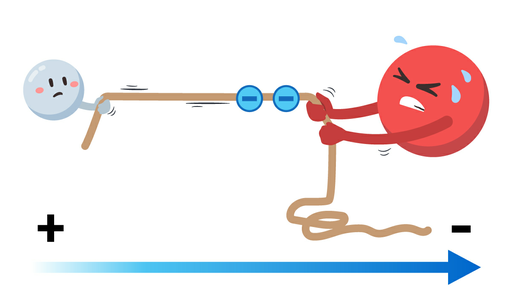
\includegraphics[width=0.8\linewidth]{water_tug}
  \begin{itemize}
  \item Sharing of electrons can lead to unequal pull
    (electronegativity)
  \end{itemize}
\end{frame}

\begin{frame}{Electronegativity Trends}
  \centering
  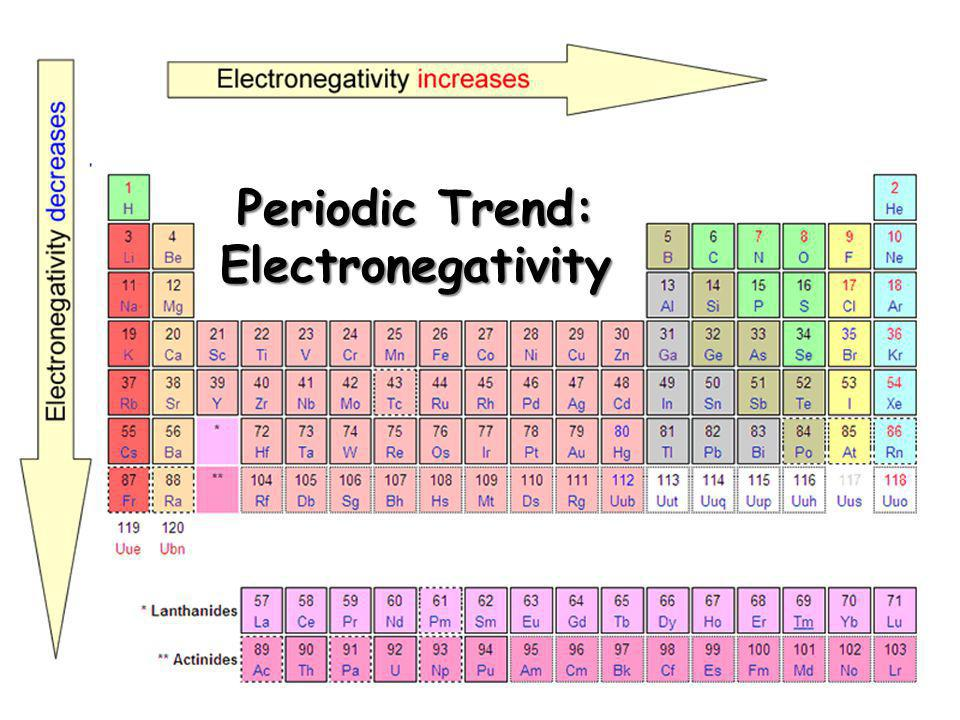
\includegraphics[width=\linewidth]{electronegativity}
\end{frame}

\section{Review: Lewis Structures}

\begin{frame}{Octet Rule}
  \textbf{Octet Rule} - Atoms have a tendency to achieve
  an electron configuration having 8 valence electrons

  \textbf{Q:} How many electrons are needed for the following
  atoms to achieve the octet rule: C, N, O, F, Xe, and Ne
\end{frame}

\begin{frame}{Exception to Octet Rule}
  \begin{center}
    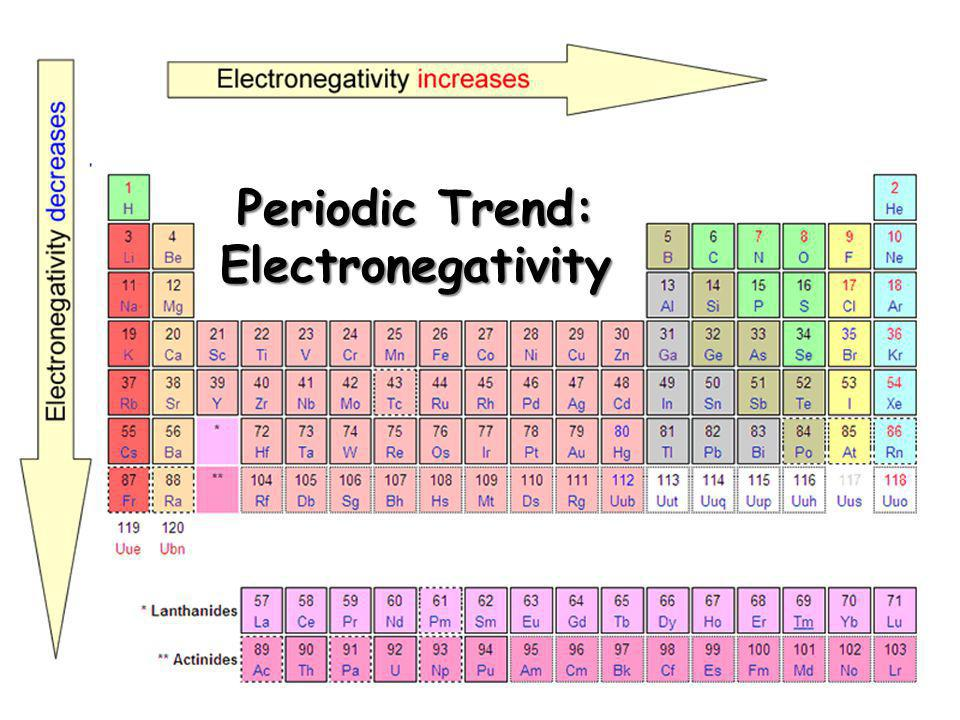
\includegraphics[width=0.75\linewidth]{electronegativity}
  \end{center}
  
  \textit{Exceptions:} Atoms starting in the
    3rd row can break the octet rule

  \textbf{Q:} Why are these atoms able to break
    the octet rule?
\end{frame}

\begin{frame}{Drawing Lewis Structures}
  \begin{enumerate}
  \item Count the total number of valence electrons
  \item Draw the atomic skeleton by determining the central atoms
    (generally the one capable of making many bonds)
  \item Add single bonds (each counts as 2 electrons) to atoms
    and add lone pairs if needed to satisfy the octet rule
  \item Check that if the amount of valence electrons counted match
    the Lewis structure
  \item Check formal charges on the atoms
  \end{enumerate}
\end{frame}

\begin{frame}{Computing Formal Charges}
  \begin{center}
    Formal Charge = VE - $\frac{1}{2}$ BE - NBE
  \end{center}
  where VE is the number of valence electrons, BE is the bonding
  electron, and NBE is the nonbonding electron aka lone pairs
\end{frame}

\begin{frame}{Resonance Structures}
  \textbf{Resonance structures} - the movement of electrons satisfying
  a valid Lewis Structure
  
  \begin{center}
    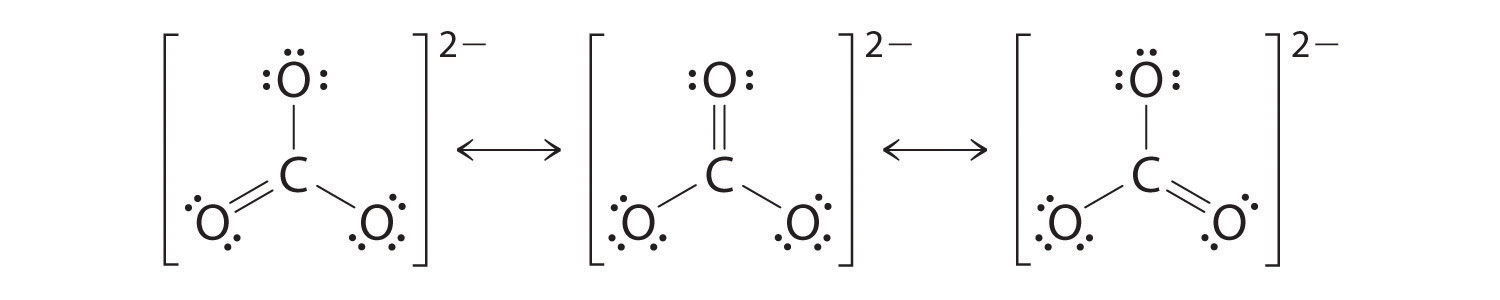
\includegraphics[width=1\linewidth]{resonance_struct}
  \end{center}
  
  \textbf{Q:} What are the formal charges for the atoms in CO$_3^{2-}$?
\end{frame}

\section{Functional Groups}

\begin{frame}{Functional Groups in Hydrocarbons}
  \textbf{Functional Groups} - derivatives of a hydrocarbon
  \begin{center}
    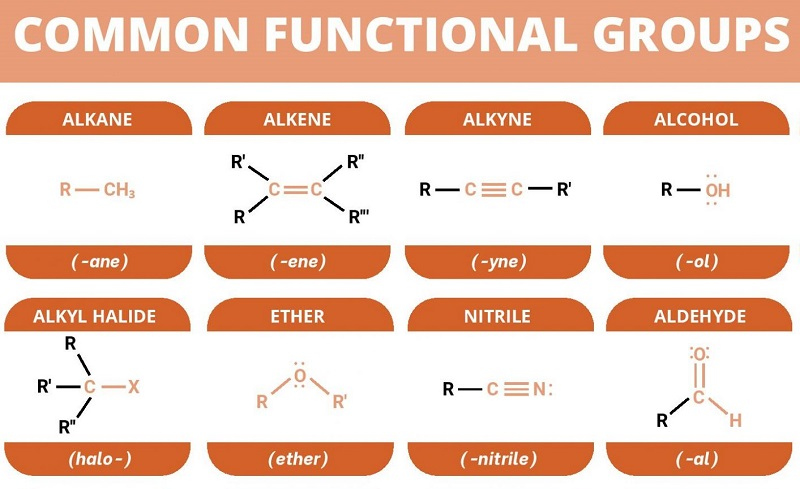
\includegraphics[width=0.8\linewidth]{func_groups}
  \end{center}
  where R represents hydrocarbon component
\end{frame}

\begin{frame}{Practice: Drawing Hydrocarbons}
  Draw the lewis structures for the following hydrocarbons:
  CH$_4$, C$_3$H$_8$, CH$_8$, C$_2$H$_2$
  \vspace{1.75in}
\end{frame}

\section{VSEPR Theory}

\begin{frame}{VSEPR Theory}
  \textbf{VSEPR Theory} - predict the geometric shape of a
  molecule or an ion; minimizes the electronic repulsion of
  the lone pairs

  Helps to determine the overall polarity of the molecule
\end{frame}

\begin{frame}
  \vspace{0.15in}
  \centering
  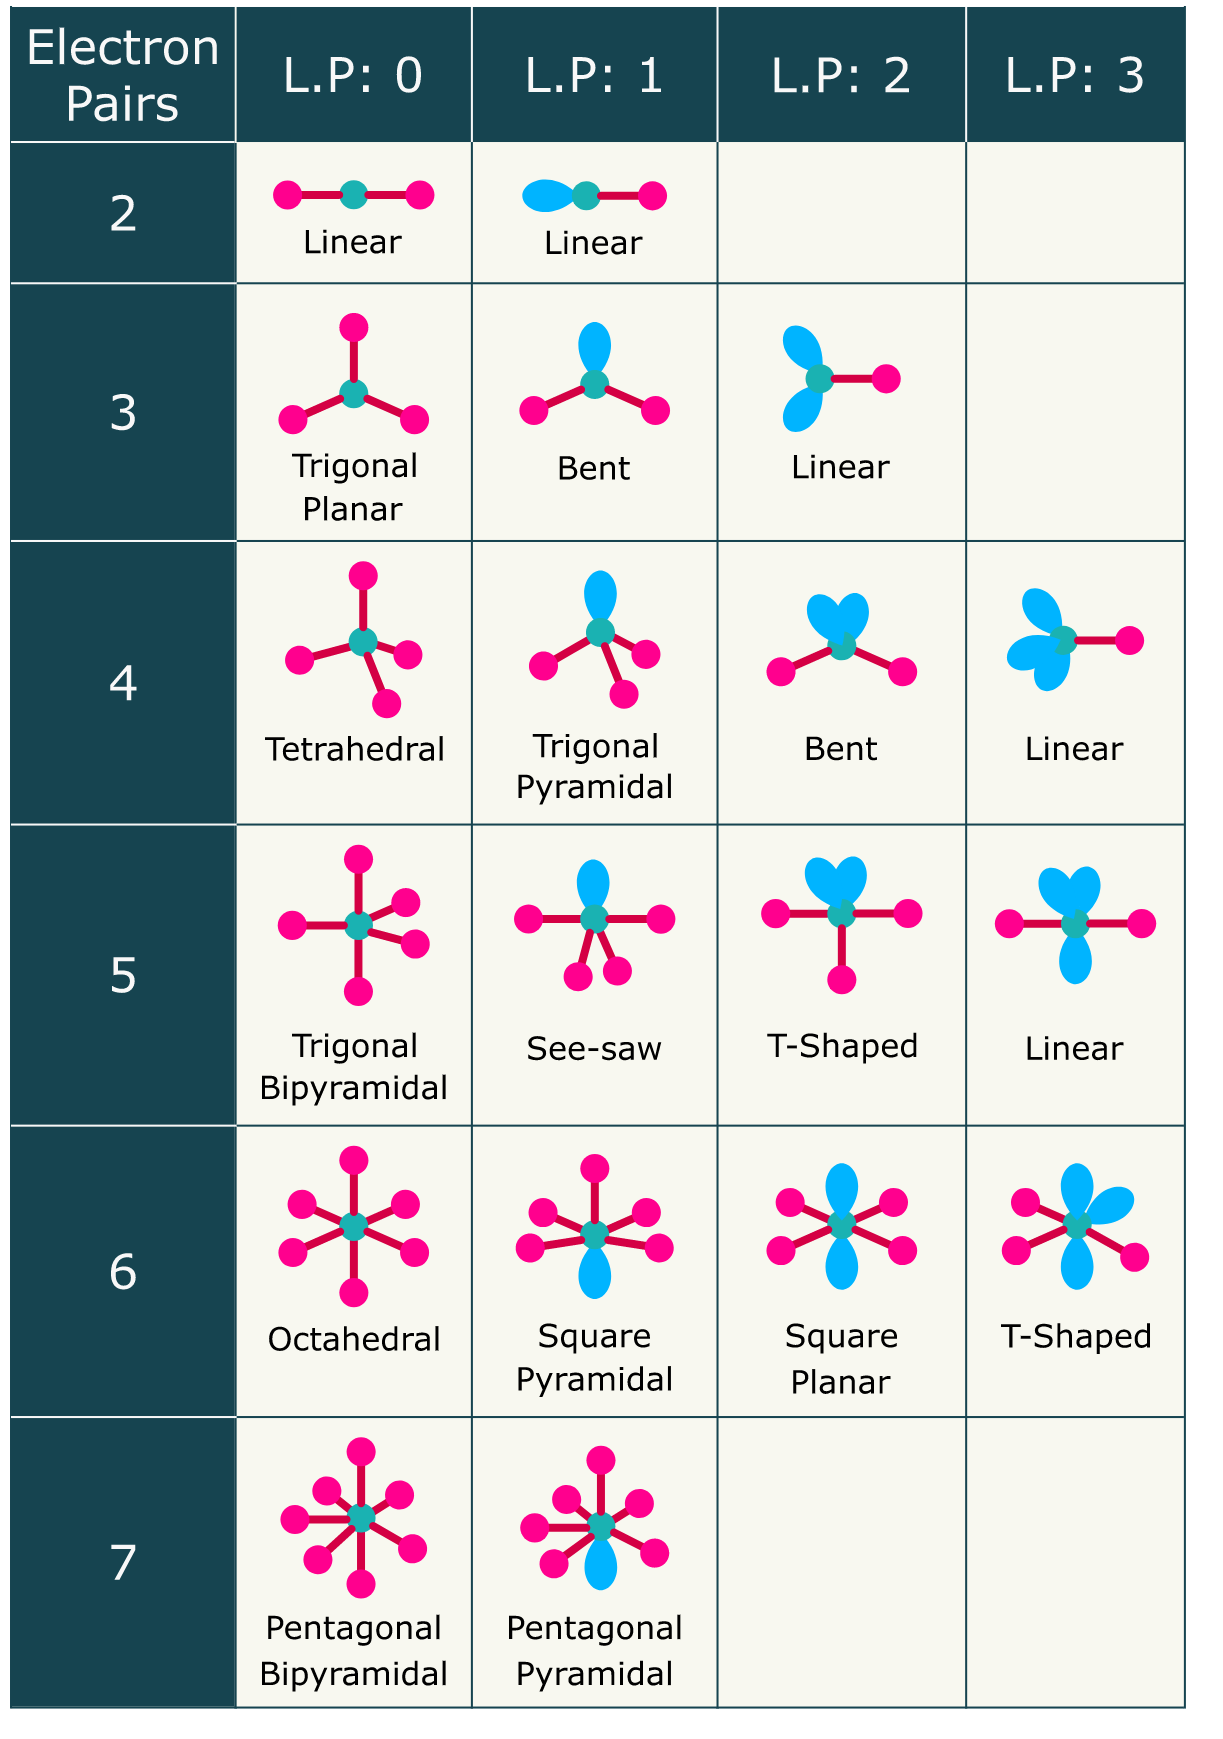
\includegraphics[width=0.6\linewidth]{vsepr_diag}
\end{frame}

\begin{frame}{Practice: Determine the Geometry}
  CO$_2$, CN, HCl, O$_3$, SO$_4^{2-}$,
  CH$_4$, C$_3$H$_8$, CH$_8$, C$_2$H$_2$
  \vspace{1.75in}
\end{frame}

\begin{frame}{Bond Polarity and Molecular Polarity}
  \begin{center}
    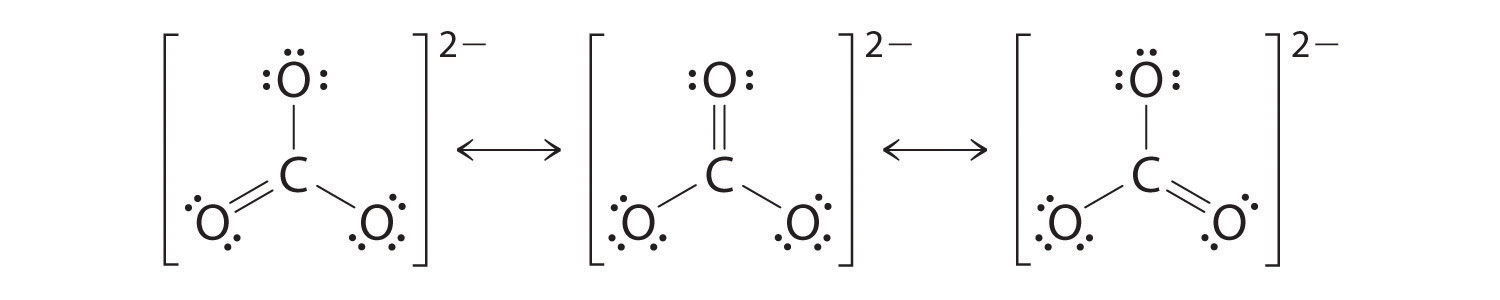
\includegraphics[width=1\linewidth]{resonance_struct}
  \end{center}

  \textbf{Q:} Is the C-O bond polar? Does this make the molecule
  overall polar?
\end{frame}

\begin{frame}{Practice: Classify whether Molecule is Polar}
  CO$_2$, CN, HCl, O$_3$, SO$_4^{2-}$,
  CH$_3$Cl, C$_3$H$_8$, CH$_8$, C$_2$H$_2$
  \vspace{1.75in}
\end{frame}

\end{document}
